\documentclass[12pt,a4paper]{scrartcl}
\usepackage[utf8]{inputenc}
%\usepackage[ngerman]{babel}
\usepackage{amsmath}
\usepackage{amssymb}
\usepackage{tabularx}
\usepackage{graphicx}
\usepackage{color}
\usepackage{hyperref}

\parskip 12pt
\parindent 0pt
\renewcommand{\labelenumi}{\alph{enumi})}
\renewcommand{\labelenumii}{\arabic{enumii})}

\definecolor{darkblue}{rgb}{0,0,.5}
\hypersetup{
  pdftitle={Helix Script},
  pdfauthor={TroY},
  colorlinks=true,
  breaklinks=true,
  linkcolor=black,
  menucolor=black,
  pagecolor=black,
  urlcolor=darkblue
}

% Setzt Zeilenabstand in align-Umgebungen:
\setlength{\jot}{12pt}

\begin{document}

	\begin{center}
		\begin{LARGE}
			\textbf{Helix Script 0.3}
		\end{LARGE}
		
		\textbf{Extract Object Collections 0.1.2}

		\textit{- TroY, March 2008 -} \\
		\textit{\href{http://www.uninformativ.de}{uninformativ.de}}
	\end{center}
	
\bigskip

\tableofcontents

\pagebreak

\section{Introduction}
The helix script allows you to easily create spirals winding around
an arbitrary curve with Art of Illusion. Pictures say more than a
thousand words:

\begin{center}
	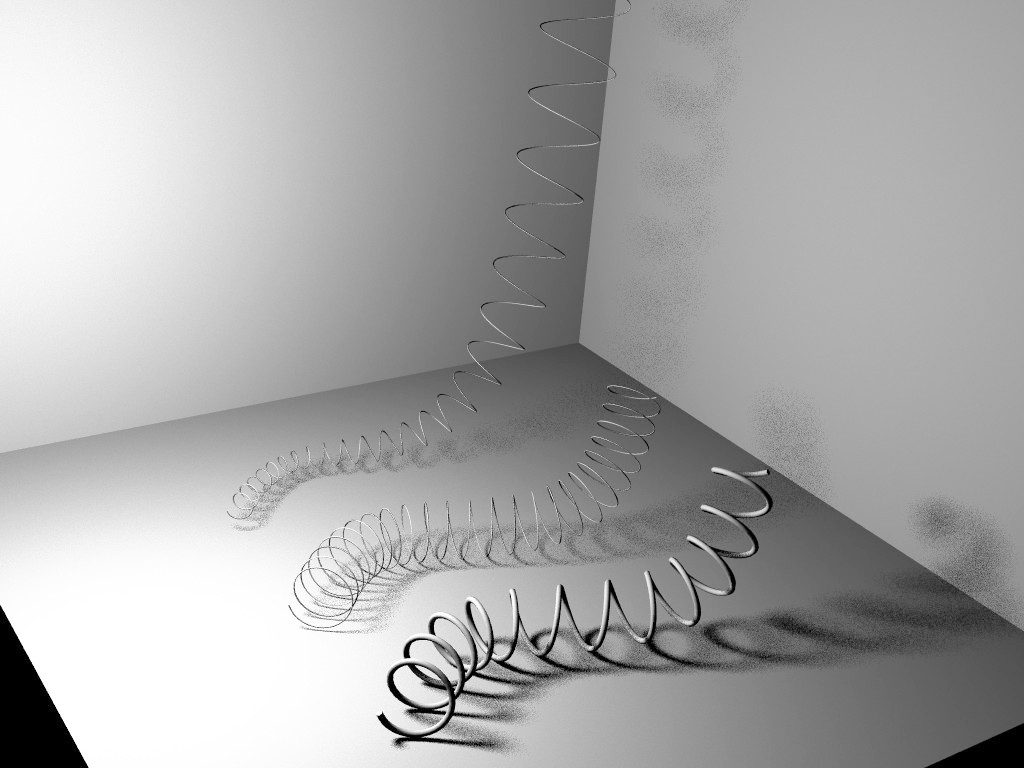
\includegraphics[width=0.75\textwidth]{../pics/presentation-bright.jpg}
\end{center}

You could use such helices as telephone wires, tubes for trucks,
DNS strings, a ring-tailed pig or whatever.

As you can see, the helix is variable in its \emph{density},
\emph{thickness} and \emph{radius} - the radius can also be influenced
\emph{later on in the spiral}. The final product can be a tube or another
raw curve on which you can do further work.

In contrast to version 0.1, now there's only one way to create a helix:
as a \emph{scripted object}. So, the spirals parameters remain editable
all the time as well as the spiral itself is permanently based on its
trajectory\footnote{I used the word ``trajectory'' here
as it makes more sense - but we're talking about common primitve curves,
you don't have to use the trajectory-script.} (basis for an animation).

If you want to use the curve/tube created by the script as common objects,
you can now use the \emph{Extract Object Collections Tool} - which is
delivered as a separate script (see last chapter).

\section{Installation}
Installation is very easy:
\begin{itemize}
	\item \texttt{Helix.bsh} goes into the \texttt{Scripts/Objects} -
	subdirectory of your Art of Illusion-directory
	\item \texttt{ExtractObjectCollections.bsh} goes into the \texttt{Scripts/Tools} -
	subdirectory of your Art of Illusion-directory
\end{itemize}
If you had AoI running during that process, you should restart it
before trying to use the scripts.

\section{Creating a Helix}
Usually, you first have to create a trajectory as a regular curve.
After that, you have to add a ``Scripted Object'' to your scene, so
choose ``Tools'', ``Created Scripted Object''. A new window pops up
where you have to enter a name for the script, also choose ``Helix''
in the dropdown list. The next window shows the script itself - that's
the point where the spirals parameters will be set:
\begin{center}
	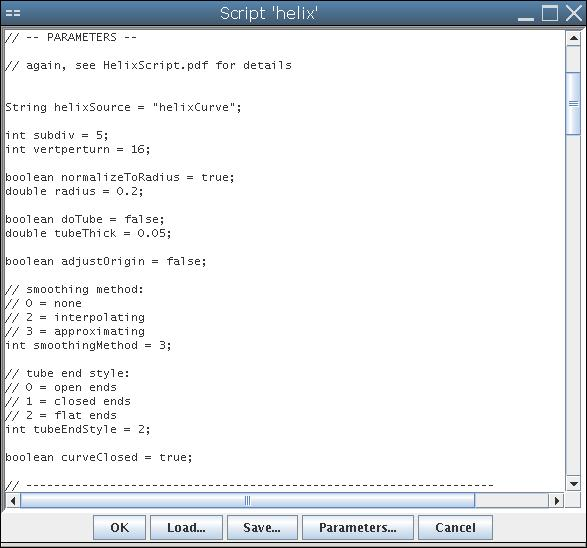
\includegraphics[width=0.5\textwidth]{../pics/createSO.jpg}
\end{center}
Keep an eye on the parameter \texttt{helixSource}: It's the name of the
trajectory you want to apply the script on. The default value is
``helixCurve'' - you have to rename your curve or change this parameter
so the script can find it. Of course, if you want to create several
spirals, all of them have to have different names.

Don't care about the code below the line full of dashes.

\section{Parameters}
\subsection{Source Object: \texttt{helixSource}}
As mentioned above, the parameter \texttt{helixSource} is set to the
name of the object which will be the trajectory - it'll describe the
path for the helix to be built around.

This object does not have to be a primitive \emph{Curve} but can also
be a \emph{Tube} or even another \emph{Object Collection}.

In Art of Illusion, Object Collections are generic\footnote{Not ``generic''
as in ``Java Generics''. ;)} containers which can hold any number and
any type of objects. The most common collections may be \emph{Scripted
Objects}, but the \emph{Tree and Plant Designer} creates such objects
as well.

This means:
\begin{itemize}
	\item Helices can be built using arbitrary curves ...
	\item ... but you can use tubes as well. The first idea which
		comes to my mind is using the \emph{Coil Envelope}-Script as the
		base for a helix as it creates a tube.\footnote{Actually, it's
		an object collection, but it only contains a single tube.}
	\item It's possible to use one helix script as a base for another
		helix without having to extract the curve first. This way,
		you can easily and quickly create ``double helices''.
	\item You can use TaPD-objects as a base - but there's a limitation:
		The helix script uses the very first curve it finds inside an
		object collection. In most cases this will be the plants stem.
		
		\textbf{Note:} You can use the extraction script to convert a
		whole TaPD-object into several common objects. After you've done that,
		you can use one of the newly created tubes as a base for a helix
		and delete the other ones.
\end{itemize}

An example for cascading two helix scripts is shown in chapter 5.

\subsection{Number of Subdivisions: \texttt{subdiv}}
Sets the number of subdivisions which will be applied to the trajectory
before creating the helix (this won't alter the original curve, it's
just temporary). The spiral will be built with this subdivided curve,
so you can control the spiral's \emph{density} with this parameter:
The more subdivisions you have, the more dense your helix will be.

Additionally, the trajectory's density will have the same influence.
As you can see below, there are more vertices in the lower left than
in the upper right - the helix adopts this density:
\begin{center}
	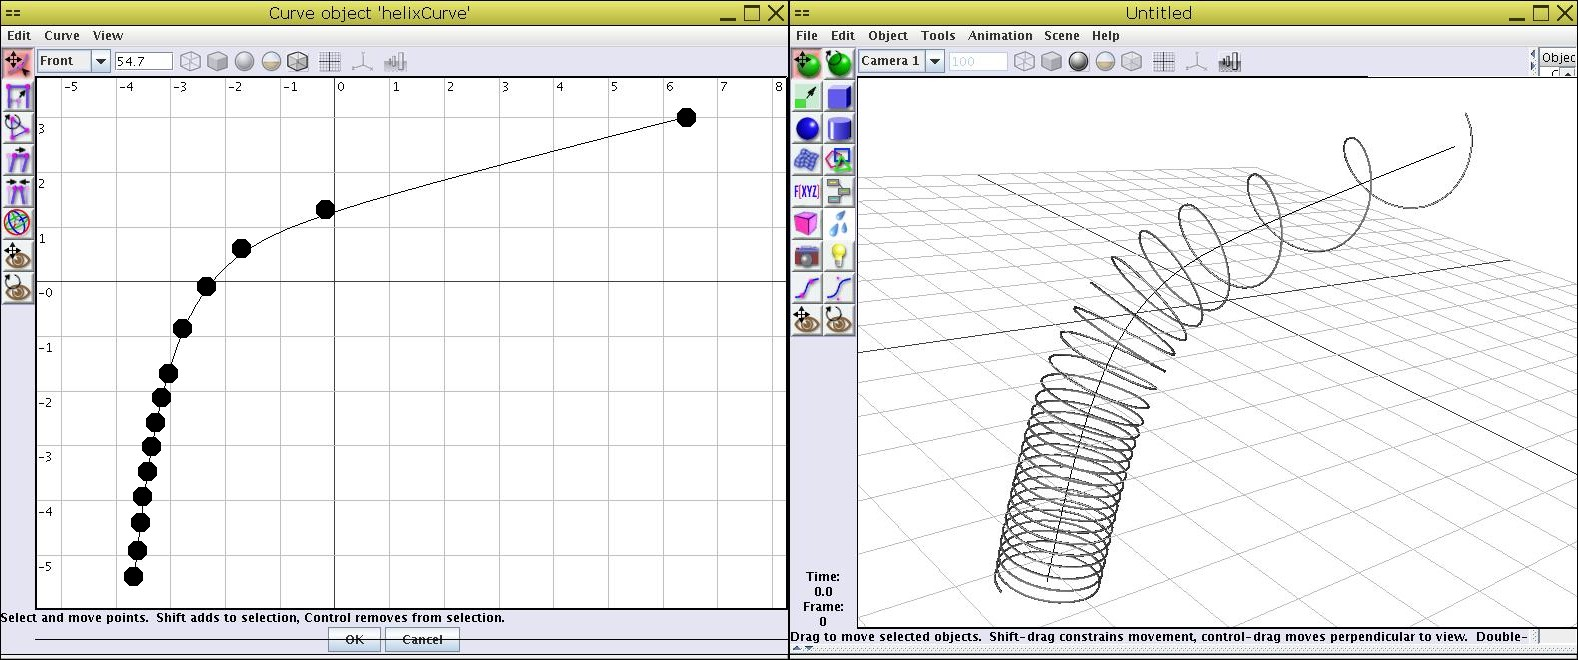
\includegraphics[width=0.75\textwidth]{../pics/dichte-comp-1.jpg}
\end{center}

\textbf{Warning:} This setting controls the number of times where the
amount of vertices is \textbf{doubled}! This means, if set to 6, your
subdivided trajectory will have twice the points in comparison with a
value of 5. Accordingly, it takes a lot of time to build a spiral on
a trajectory which is divided too much.

\subsection{Vertices per Turn: \texttt{vertperturn}}
This one is trivial: It sets the number of vertices you want to have
per turn. More vertices means a more ``round'' result but also longer
to compute.

\subsection{Radius Normalization (\texttt{normalizeToRadius}) and Radius (\texttt{radius})}
With activated normaliziation, your spiral will have the given radius
all the time. If it's disabled, the density of the vertices on the
trajectory will influence the helix' radius - in this case, the radius
is more an approximate value than an exact value. Additionally, you'd
have to increase its value by 10 or 100 to get a similar real radius
(in comparison to normalization).

\pagebreak

This is how the spiral above will look like with deactivated normalization:
\begin{center}
	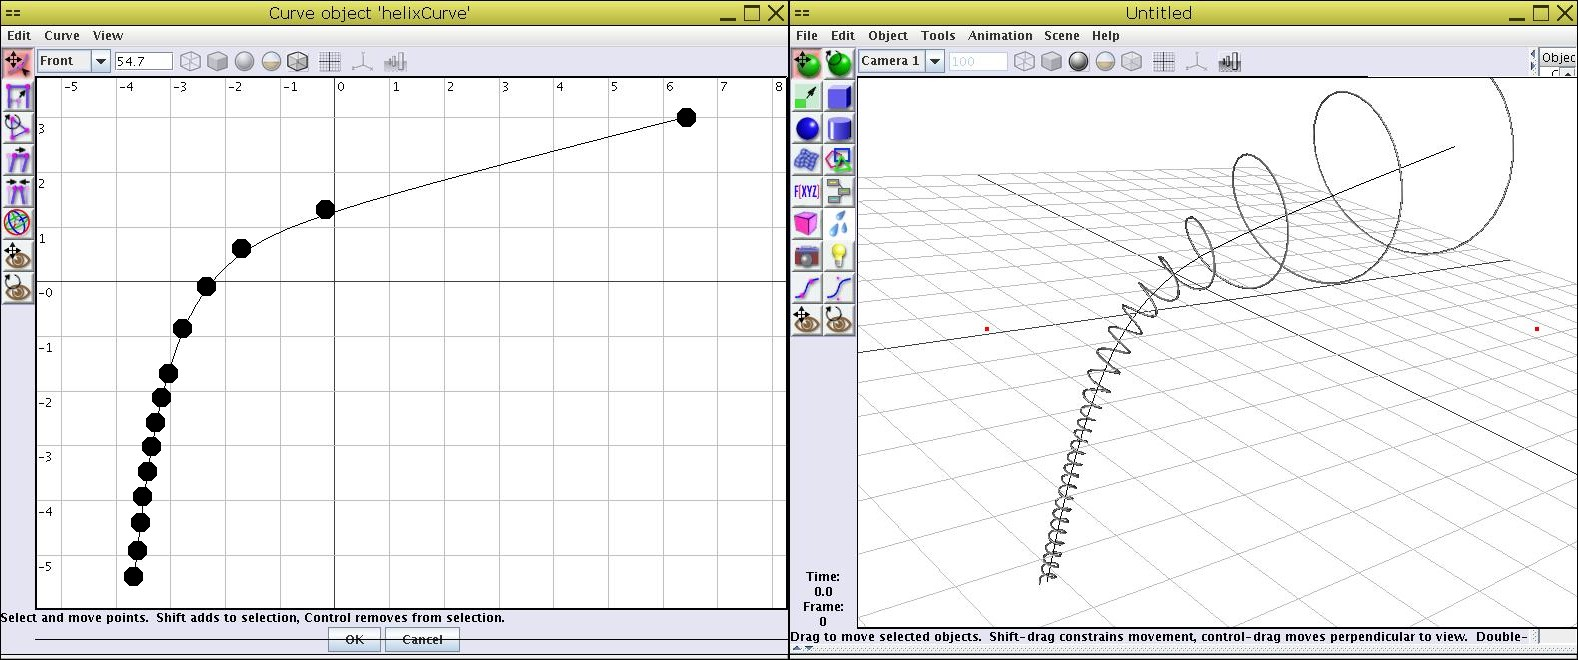
\includegraphics[width=0.75\textwidth]{../pics/dichte-comp-2.jpg}
\end{center}

\subsection{Create a Tube (\texttt{doTube}) and Tube Thickness (\texttt{tubeThickness})}
These are self-explaining again: Do you want to create a raw curve or
a tube? If you choose the latter, you can set its thickness. That's all.

\subsection{Thickness Tapering: \texttt{thickTapering}}
If you're creating a tube and if radius normalization is \emph{disabled},
you can choose whether to enable thickness tapering or not. Depending
on the current radius of the spiral it will reduce the thickness of the
tube.

Tapering disabled (upper tube) and enabled (lower tube):
\begin{center}
	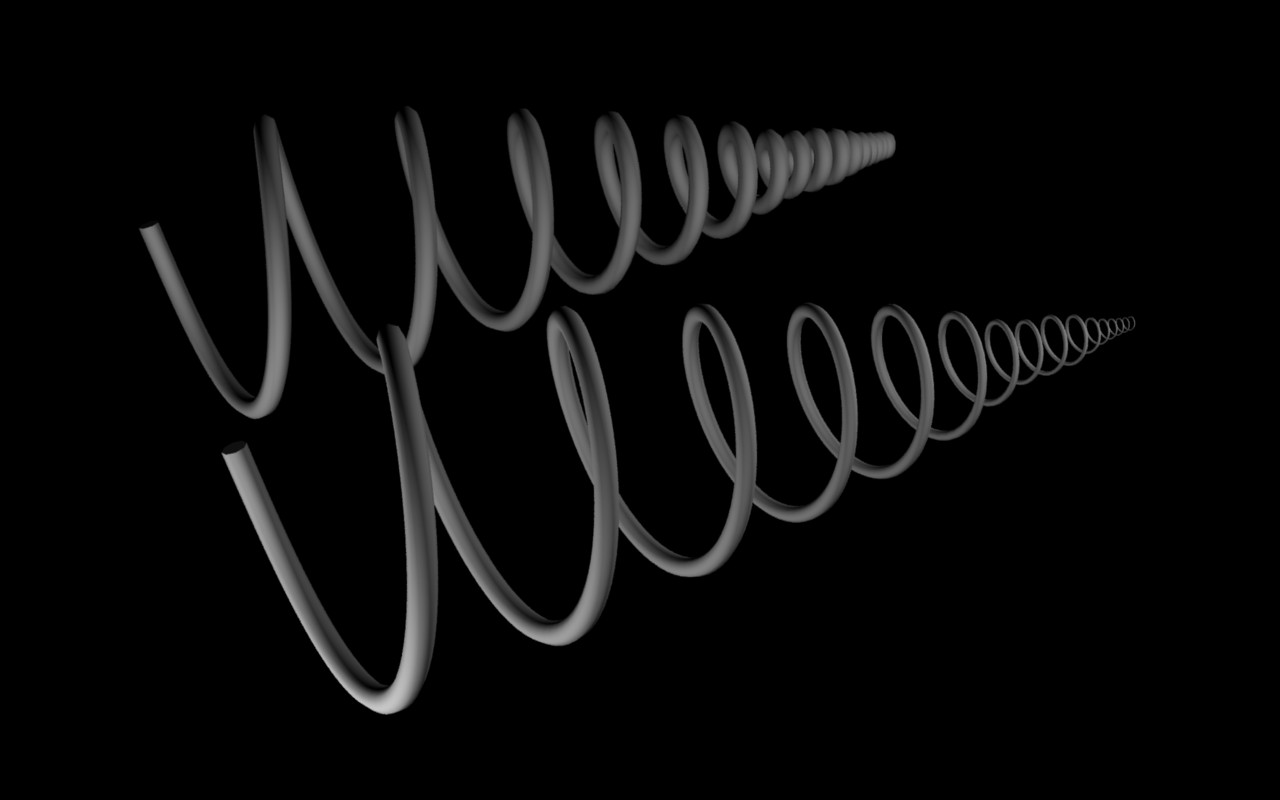
\includegraphics[width=0.75\textwidth]{../pics/thicknessTapering.jpg}
\end{center}

\subsection{Adjust Object's Origin: \texttt{adjustOrigin}}
By setting this parameter to \texttt{true}, the script will adjust its own
position and rotation to match the location of the base object. So,
the helix will always wind around its trajectory.

Setting it to \texttt{false} results in the script being freely moveable
- its initial position will be (0, 0, 0).

You can derive the reason why the default setting is \texttt{false}:
Activating this option means that the script is not moveable. It will
always jump back to the position of its base.

\subsection{Common Parameters: \texttt{smoothingMethod}, \texttt{tubeEndStyle}, \texttt{curveClosed}}
As with common curves and tubes, this parameters set how the object
will be smoothed and - if you create a tube - what kind of tube ends
you'd like to have. If you just create a curve, the parameter ``curveClosed''
obviously controls whether the curve will be closed or not.

You can set this numerical values:

\underline{\texttt{smoothingMethod}}
\begin{itemize}
	\item 0 = No smoothing
	\item 2 = Interpolating
	\item 3 = Approximating
\end{itemize}

\underline{\texttt{tubeEndStyle}}
\begin{itemize}
	\item 0 = Open ends (results in a hollow tube)
	\item 1 = Connected ends (same as \texttt{curveClosed = true} when
		using a curve)
	\item 2 = Flat ends, unconnected
\end{itemize}

\subsection{Glitch Correction (\texttt{glitchCorrection})}
Sadly, in some situations glitches may appear. On the one hand, this
happens due to limited accuracy of todays computers, on the other hand,
it's a flaw of my routine calculating the helix.

The helix on the left has \texttt{glitchCorrection} set to 1 whereas
the helix on the right has \texttt{glitchCorrection} set to -1. Actually,
\texttt{glitchCorrection} is a factor representing the sign of an angle
and that's why only values of 1 or -1 make sense.
\begin{center}
	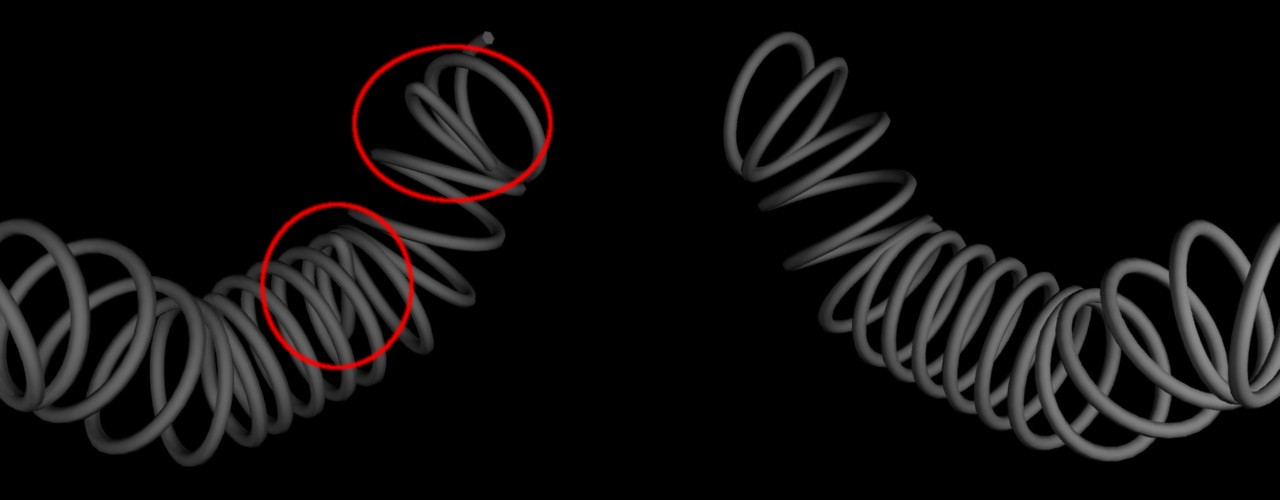
\includegraphics[width=0.75\textwidth]{../pics/glitchCorr-edit.jpg}
\end{center}

As you can see, in the left spiral two glitches appear which are
eliminated in the right spiral.

\subsection{Spiral Offset (\texttt{spiralOffset})}
This parameter determines the amount of degree after which the spiral
will start. For example, set this to ``180.0'' in order to ``flip''
the spiral around the curve.

\section{Animating Helices}
Since Art of Illusion 2.6, you can animate primitive curves and tubes.
It's just the same as animating any other object in Art of Illusion,
so if you encounter any strange problems or if you're missing the basics,
head over to the \href{http://www.housepixels.com/aoimanual/contents.html}{AoI Documentation}.

Anyway, here's a short example.
\begin{itemize}
	\item Given an arbitrary curve, you have to convert it to an actor -
		this means, you won't be able anymore to add or delete points
		on the curve, but now you can add poses to it. Do so by choosing
		``Object'', ``Convert to Actor''.
	\item Double click on the curve in order to add some poses.
	\item Add a \emph{Pose Track} to your curve: Select it and choose
		``Animation'', ``Add Track to Selected Object'', ``Pose''.
	\item Add some keyframes.
	\item Add a Helix Script to your scene and set \texttt{helixSource}
		to the curves name.
	\item Move the pointer on the score and see how the spiral will
		bend.
\end{itemize}

\begin{center}
	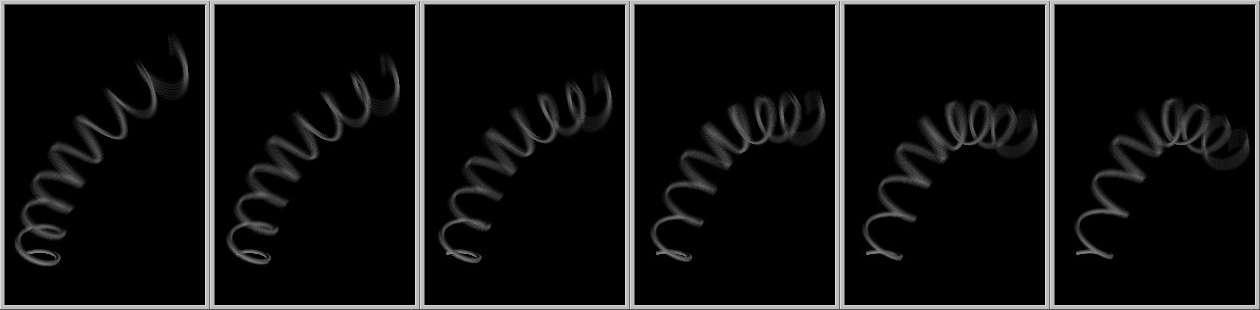
\includegraphics[width=0.75\textwidth]{../pics/helixAni.jpg}
\end{center}

When rendering animated helices, \emph{Motion Blur} is a very nice
feature.

\subsection{Using dynamic Parameters in Animations}
You can additionally add a pose track to the script itself. This allows
you to change some parameters by time: \texttt{radius},
\texttt{tubeThick}, \texttt{spiralOffset} and \texttt{glitchCorrection}.

The script will have a look to see if you created any parameters. If not,
it uses the static values you set directly in the script.

How to add dynamic parameters:
\begin{itemize}
	\item Double click on the script to bring up its editor window
	\item Click on ``Parameters...''
	\item Click on ``Add'', so a new parameter will be created
	\item Name it just as the parameters in the script: ``radius'',
		``tubeThick'' or whatever (this is case sensitive)
	\item Enter a default value and click ``OK''
	\item Now you can add a pose track to the script - add a keyframe
		and double click on it: You'll see that you can change the
		values of the parameters you just added to the script.
\end{itemize}

However, \texttt{glitchCorrection} translates the values in a slight
different way: A keyframe with \texttt{glitchCorrection} set to ``1.0''
means the internal integer value of this parameter is set to ``1'',
whereas anything else sets it to ``-1''.

\section{Cascading Helices}
Here's a step-by-step example (nearly) on how to cascade two helix
scripts.

\begin{enumerate}
	\item Create an arbitrary curve which will function as the trajectory
		for the first script. Name it ``helixCurve'' to skip the renaming
		part later.
	\item As described above, add a new helix script as a
		\emph{scripted object}. Name this script ``helixScript1''.
	\item Do some manual fine tuning of the trajectory. Just think of
		how it would look like when another helix would be built on
		top of this first helix - adjust subdivision and radius
		accordingly. Radius normalization should be activated.
	\item Insert a second helix script. This time set its parameter
		\texttt{helixSource} to ``helixScript1''. Now this second script
		has the order to look inside the first script, use its tube
		and build its own helix around that tube.
\end{enumerate}

This is how it could look like:

\begin{center}
	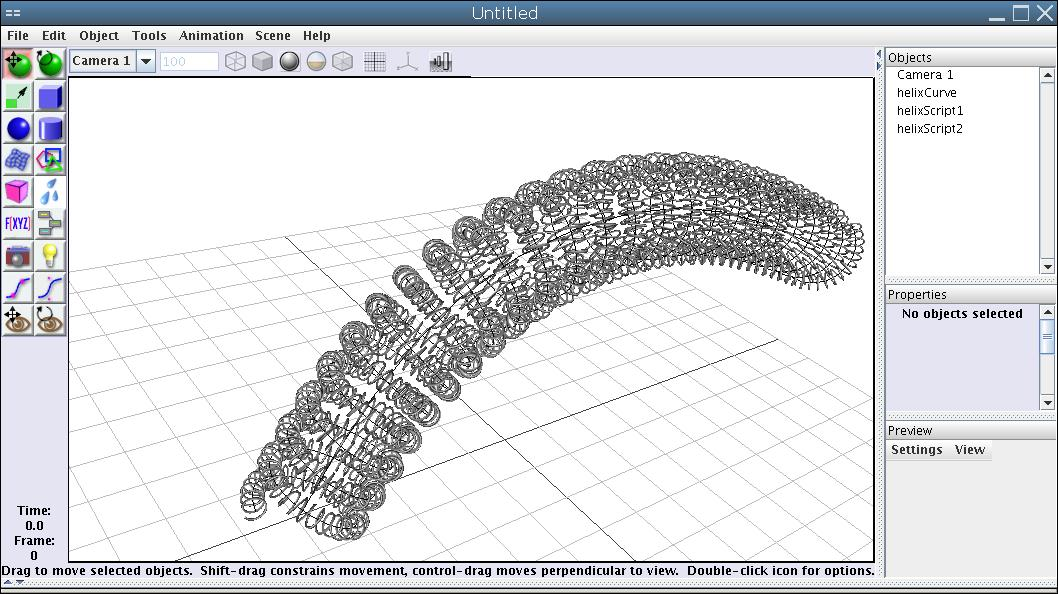
\includegraphics[width=0.75\textwidth]{../pics/doubleHelix.jpg}
\end{center}

\section{Extracting objects out of \texttt{Object Collections}}
With the script \texttt{ExtractObjectCollections.bsh} you can extract
all objects of an object collection. It doesn't matter what kind of
object collection it is - can be a scripted object or anything else.

To perform the extraction, you have to select all your objects - you
can select several object collections at one time, they will be 
deconstructed one by one\footnote{They won't be deleted or changed.}.
After that, choose ``Tools'', ``Scripts'', ``ExtractObjectCollections''.
If you have selected invalid objects (means no object collections), you
will be informed about that, but other remaining objects will be tried
to be deconstructed as well.

The found objects will be grouped - and named according to their type:
``Sphere 1'', ``Sphere 2'', ``Tube 3'' and so on.

All extracted objects will reside at the same location in the scene
as their parent objects, also rotation will be adopted. Textures
and materials are copied if they do not yet exist in the scene (this is
the case if you want to extract TaPD-objects).

\section{Changelog}
\subsection{Helix}
\underline{0.3}
\begin{itemize}
	\item Added a correction routine to reduce glitches
	\item Got ready for animation (now accepts actors and extracts the
		curve/tube)
	\item Dynamic parameters: \texttt{radius}, \texttt{tubeThick},
		\texttt{spiralOffset} and \texttt{glitchCorrection}
	\item Introduced thickness tapering
\end{itemize}
\underline{0.2}
\begin{itemize}
	\item Removed the ``tool'' version
	\item Accepts tubes as input
	\item Accepts any kind of object collections as input - the first
		curve or tube in that collection is used
	\item If requested adoption of position and rotation of base objects
	\item Added \texttt{smoothingMethod}, \texttt{tubeEndStyle} and
		\texttt{curveClosed}
\end{itemize}

\subsection{Extract Object Collections}
\underline{0.1.2}
\begin{itemize}
	\item Generalization so that every object collection can be used
	\item Textures and materials are copied from the objects in the
		container (they were copied from the container itself before)
	\item Textures and materials which do not yet exist in the scene
		are added to it
\end{itemize}

\end{document}
